\begin{frame}[noframenumbering]
\vfill
\begin{center}
\begin{beamercolorbox}[sep=8pt,center]{title}
\usebeamerfont{title}
Backup-Folien
\end{beamercolorbox}
\end{center}
\vfill
\end{frame}

\begin{frame}[noframenumbering]
\frametitle{Entscheidungsmodell: RCPSP\only<2>{-OC}}
\begin{footnotesize}
\begin{itemize}
\item Zielfunktion\\[-7mm]
\[
		\only<1>{\mbox{min } \sum_{t=EFT_{J+1}}^{LFT_{J+1}} t \cdot x_{{J+1},t} \textcolor{white}{\enspace - \sum_{r \in \mathcal{R}} \sum_{t \in \mathcal{T}} \kappa_r \cdot z_{rt}}}\only<2>{\textcolor{red}{\mbox{max } \sum_{t=EFT_{J+1}}^{LFT_{J+1}} u_t \cdot x_{{J+1},t} - \sum_{r \in \mathcal{R}} \sum_{t \in \mathcal{T}} \kappa_r \cdot z_{rt}}}
\]

\item Einmalige Durchführung
\[
\sum_{t=EFT_j}^{LFT_j} x_{jt} = 1 \,\,\,\quad\quad\quad\quad\quad\quad\quad\quad\quad\quad\quad j \in \mathcal{J}\textcolor{white}{, t \in \mathcal{T}}
\]

\item Reihenfolgerestriktionen
\[
\sum_{t=EFT_i}^{LFT_i} x_{it} \cdot t \leq \sum_{t=EFT_j}^{LFT_j} x_{jt} \cdot t - d_j \,\,\:\:\:\quad\quad\quad j \in \mathcal{J}, \; i \in \mathcal{P}_j
\]

\item Kapazitätsrestriktionen
\[
\sum_{j=1}^{J} \sum_{\tau=t}^{t+d_j-1} k_{jr} \cdot x_{j\tau} \leq K_r\only<1>{\textcolor{white}{ + z_{rt}}}\only<2>{ \textcolor{red}{+ z_{rt}}} \,\,\:\:\:\:\:\quad\quad\quad\quad r \in \mathcal{R}, \; t \in \mathcal{T}
\]

\item<2> Obere Schranke für Zusatzkapazität\\[-3mm]
\[
\textcolor{red}{z_{rt} \leq \overline{z}_r} \,\;\;\quad\quad\quad\quad\quad\quad\quad\quad\quad\quad\quad\quad\quad\quad r \in \mathcal{R}, \; t \in \mathcal{T}
\]
\end{itemize}
\end{footnotesize}
\end{frame}

%%%%%%%%%%%%%%%%%%%%%%%%%%%%%%%%%%%%%%%%%%%%%%%%%%%%%%%%%%%%%%%%%%%%%%%%%%%%%%%%%%%%%%%%%%%

\begin{frame}[noframenumbering]
\frametitle{Verwandte Probleme aus der Literatur}
\begin{itemize}
\item Variable Kapazitäten
\begin{itemize}
\item Ressourcenprofil als Parameter {\footnotesize \cite{Klein2000}, \cite{Hartmann2012}}
\item Ressourceninvestitionsproblem {\footnotesize \cite{Mohring1984}}
\item Ressourcenabweichungsproblem {\footnotesize \cite{Neumann2003}} 
\item Ressourcenüberladungsproblem {\footnotesize \cite{Neumann2003}}
\end{itemize}
\vspace*{4mm}
\item Variable Ressourcennachfrage
\begin{itemize}
\item Flexible Ressourcenprofile {\footnotesize \cite{Ranjbar2010}}
\item Zeit-Kosten-Tradeoff-Problem {\footnotesize \cite{Demeulemeester1996}}
\end{itemize}
\end{itemize}

\end{frame}

%%%%%%%%%%%%%%%%%%%%%%%%%%%%%%%%%%%%%%%%%%%%%%%%%%%%%%%%%%%%%%%%%%%%%%%%%%%%%%%%%%%%%%%%%%%%%%%

\begin{frame}[noframenumbering]
\frametitle{Gemeinsamkeiten der GAs (\only<1>{1}\only<2>{2}/2)}

\only<1>{
\begin{itemize}
\item Aktivitätenliste $\lambda$ als Bestandteil der Repräsentation
\item Initialpopulation

\begin{itemize}\item Regret-Based Biased Random Sampling\end{itemize}
\item Kreuzung
	\begin{itemize}
	\item Paarbildung:\\Ziehe zufälliges Paar noch nicht gewählter Individuen\\[4mm]
	\item Tochter (Sohn) per One Point Crossover, d.h.:
	\item[] Übernehme bis zufälliger Stelle $q$ von der Mutter (Vater), Rest in Reihenfolge vom Vater (Mutter)
	\end{itemize}
\end{itemize}
}
\only<2>{
\begin{itemize}
\item Mutation
\begin{itemize}\item Mit Wahrscheinlichkeit $P_{mutate}$ vertausche AG mit Nachbarn, falls zulässig (Swap Neighborhood)\\[3mm]\end{itemize}
\item Selektion
\begin{itemize}\item Sortiere Gesamtpopulation (Eltern \& Kinder) nach absteigender Fitness. Neue Elterngeneration ist ``vordere'' Hälfte (Ranking Method)\\[3mm]\end{itemize}
\item Fitness \begin{itemize}\item DB von durch Individuum per SSGS induziertem Plan\end{itemize}
\end{itemize}
}
\end{frame}

%%%%%%%%%%%%%%%%%%%%%%%%%%%%%%%%%%%%%%%%%%%%%%%%%%%%%%%%%%%%%%%%%%%%%%%%%%%%%%%%%%%%%%%%%%%%%%%%

\begin{frame}[noframenumbering]
\frametitle{Bestimmte Zusatzkapazität je\\Ressource und Periode erlauben}
\begin{itemize}
\item Aktivitätenliste um $\tilde{z}_{rt} \in \{0, \ldots, \overline{z}_r \}$ erweitern
\item Für Ressourcenzulässigkeit in SGS zur Verfügung stehende Kapazität: Normalkapazität + $\tilde{z}_{rt}$
\item Möglicher Gebrauch von Überstunden über Planungshorizont \textcolor{red}{\emph{flexibel}}
\end{itemize}

\begin{small}
\begin{center}
\begin{tabular}{rl}
\hline 
Individuum & $(\lambda|\tilde{z}_{rt})=(0,1,3,2,4|\begin{pmatrix} 0 & 2 & 2 & \ldots\\ \vdots & \ddots \end{pmatrix})$\parbox[c][40pt][c]{0pt}{}\tabularnewline
\hline 
Initialpopulation & $\tilde{z}_{rt}=\mbox{rand }0\ldots\overline{z}_{r}\;\forall r,t$\tabularnewline
\hline 
Rekombination & One Point Crossover\tabularnewline
\hline 
Mutation & $\tilde{z}_{rt}=\mbox{rand }0\ldots\overline{z}_{r}$ mit $P_{mutate}$\tabularnewline
\hline 
Fitness & DB von Plan erzeugt durch SSGS\tabularnewline
\hline 
\end{tabular}
\end{center}
\end{small}
\end{frame}

\begin{frame}[noframenumbering]
\frametitle{Beispiel für $(\lambda|z_{rt})$:\\Einplanung von AG 2}
\includegraphics<1>[page=1, scale=0.7]{images/SSGSzrt.pdf}
\includegraphics<2>[page=2, scale=0.7]{images/SSGSzrt.pdf}
\end{frame}

\begin{frame}[noframenumbering]
\frametitle{Bestimmte Zusatzkapazität je\\Ressource erlauben}

\begin{itemize}
\item Aktivitätenliste um $\tilde{z}_{r} \in \{0, \ldots, \overline{z}_r \}$ erweitern
\item Für Ressourcenzulässigkeit in SGS zur Verfügung stehende Kapazität: Normalkapazität + $\tilde{z}_{r}$
\item Möglicher Gebrauch von Überstunden über Planungshorizont \textcolor{red}{\emph{konstant}}
\end{itemize}

\begin{small}
\begin{center}
\begin{tabular}{rl}
\hline 
Individuum & $(\lambda|\tilde{z}_{r})=(0,1,3,2,4|0,2,2,0,3,2,1,\ldots)$\parbox[c][40pt][c]{0pt}{}\tabularnewline
\hline 
Initialpopulation & $\tilde{z}_{r}=\mbox{rand }0\ldots\overline{z}_{r} \; \forall r$\tabularnewline
\hline 
Rekombination & One Point Crossover\tabularnewline
\hline 
Mutation & $\tilde{z}_{r}=\mbox{rand }0\ldots\overline{z}_{r}$ mit $P_{mutate}$\tabularnewline
\hline 
Fitness & DB von Plan erzeugt durch SSGS\tabularnewline
\hline
\end{tabular}
\end{center}
\end{small}
\end{frame}

\begin{frame}[noframenumbering]
\frametitle{Beispiel für $(\lambda|z_{r})$:\\Einplanung von AG 2}
\includegraphics<1>[page=1, scale=0.7]{images/SSGSzr.pdf}
\includegraphics<2>[page=2, scale=0.7]{images/SSGSzr.pdf}
\end{frame}

%%%%%%%%%%%%%%%%%%%%%%%%%%%%%%%%%%%%%%%%%%%%%%%%%%%%%%%%%%%%%%%%%%%%%%%%%%%%%%%%%%%%%%%%%%%%%%%%%%%%%%%%%%%%%%%%%%%%%%%%

%\section{Problembibliothek}
%\begin{frame}[noframenumbering]
%\frametitle{Gliederung}
%\tableofcontents[current] %, hidesubsections]
%\end{frame}

\begin{frame}[noframenumbering]
\frametitle{Erzeugung relevanter Probleminstanzen}

\begin{itemize}
\item Obere Schranke für Zusatzkapazität $\overline{z}_r=\frac{1}{2}K_r$
\item Kostensatz für Zusatzkapazität $\kappa_r=\frac{1}{2}\mbox{GE}$
\item Projektdauerabhängiger Erlös \[u_{t}=C^{\mbox{max}} - \frac{C^{\mbox{max}}}{(T^{\mbox{max}}-T^{\mbox{min}})^2} \cdot (t-T^{\mbox{min}})^2\]
\end{itemize}

\begin{center}
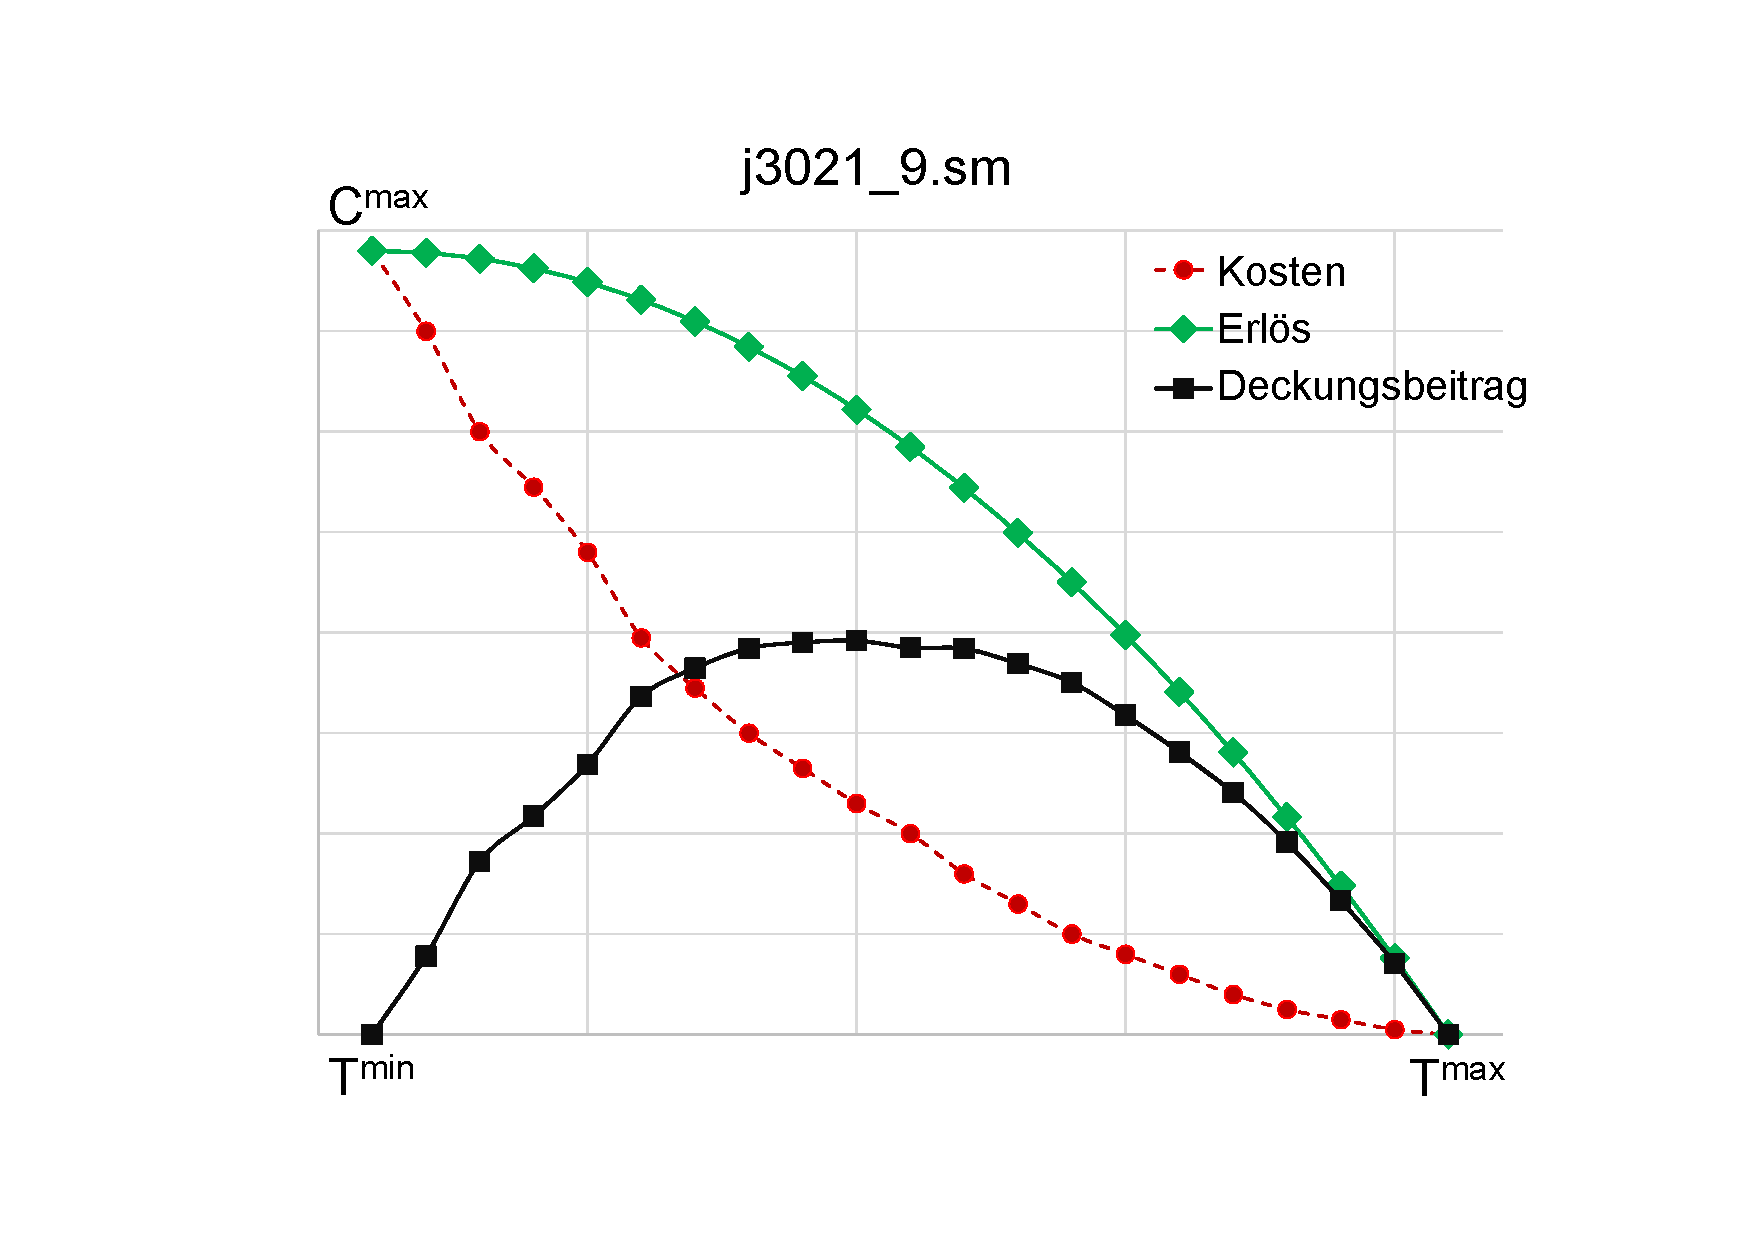
\includegraphics[scale=0.26]{images/DeadlineCosts.pdf}
\end{center}

\end{frame}


\begin{frame}[noframenumbering]
\frametitle{Parameter der Erlösfunktion}
\begin{itemize}
\item Problem: Bestimmung von $C^{\mbox{max}}$, $T^{\mbox{min}}$, $T^{\mbox{max}}$ erfordert Lösung eines RCPSP\\[5mm]
\item[$\rightarrow$]  Abschätzung mittels unterer bzw. oberer Schranken\\[2mm]
\begin{itemize}
\item $T^{\mbox{min}} \geq \mbox{max}\{EFT_{J},\mbox{max}_{r}\{\lceil\frac{\sum_{j}d_{j}k_{jr}}{K_{r}+\overline{z}_{r}}\rceil\}\}$\\[1mm]
\item $T^{\mbox{max}} \leq$ Dauer von SSGS-Ablaufplan mit $z_{rt}=0$\\[4mm]
\item $C^{\mbox{max}} \leq $ Kosten des $\mathcal{ESS}$
\end{itemize}
\end{itemize}
\end{frame}

\begin{frame}[noframenumbering]
\frametitle{Basis für Testinstanzen}
\begin{itemize}
\item Project Scheduling Problem Library (PSPLIB)
	\begin{itemize}
		\item RCPSP-Testinstanzen mit 30, 60, 90 und 120 AG
		\item Instanzgenerator PROGEN
		\item Beste bekannte Lösungen (Optimal für j30) für $T^{\mbox{max}}$\\[4mm]
	\end{itemize}

\item Erweiterung um $\kappa_r, \overline{z}_r$ und $u_t$\\[4mm]

\item Entferne Instanzen mit $T^{\mbox{min}} = T^{\mbox{max}}$
	\begin{itemize}
	\item $T^{\mbox{min}}$ kürzeste Projektdauer bei maximal möglicher ZK
	\item $T^{\mbox{max}}$ kürzeste Projektdauer bei keiner ZK
	\end{itemize}
\item Lösung von zwei RCPSPs je Testinstanz notwendig $\implies$ nur für $\lesssim 30$ AG praktikabel
\end{itemize}

\end{frame}

\begin{frame}[noframenumbering]
\frametitle{Berechnung optimaler Lösungen\\als Referenzwerte}
\begin{itemize}
\item Aktuell nur für 30 Arbeitsgänge\\[4mm]
\item GAMS-Implementierung von
	\begin{itemize}
	\item RCPSP-OC-Modell sowie
	\item RCPSP-Modell zur Berechnung von $T^{\mbox{min}}$\\[4mm]
	\end{itemize}
\item Für RCPSP-OC erweiterte j30-Testinstanzen in GDX-Format umgewandelt
\item Exakte Lösung per GUROBI parallel auf RRZN-Cluster
\item Problemspezifischer Branch\&Bound-Algorithmus
\end{itemize}
\end{frame}

\begin{frame}[noframenumbering]
\frametitle{Umsetzung der Genetischen Algorithmen}
\begin{itemize}
\item Implementierung in Delphi\\[4mm]
\item Großer Flaschenhals in $(\lambda)$-Repräsentation laut Profiling: Fitnessberechnung 
\begin{itemize}\item[$\rightarrow$] in Threads parallelisiert\\[4mm]\end{itemize}
\item Heuristik-Ausführung auf Cluster
\begin{itemize}
	\item Hoher Zeitbedarf für Gesamtevaluation:
		\begin{itemize}
		\item 12 Heuristiken
		\item 3*480 und 1*600 Projekte
		\item 1s, 2s, 10s, 15s Zeitlimit (für j30, j60, u.s.w.)
		\item[$\implies$] = $12 \cdot (480\cdot (1s + 2s + 10s) + 600\cdot15s ) = 50{,}8$ Stunden
		\end{itemize}
	\item Vergleichbarkeit
	\item Parallelisierte Berechnung gesamter Problembibliothek
\end{itemize}
\end{itemize}
\end{frame}

%%%%%%%%%%%%%%%%%%%%%%%%%%%%%%%%%%%%%%%%%%%%%%%%%%%%%%%%%%%%%%%%%%%%%%%%%%%%%%%%%%%%%%%%%%%%%%%%%%%%%%%%%

\begin{frame}[noframenumbering]
\frametitle{Konvergenzverhalten}
\includegraphics<1>[page=1, scale=0.69]{images/Convergence3011_7.pdf}
\end{frame}